\documentclass[12pt]{article}
\usepackage[utf8]{inputenc}
\usepackage{amsmath,setspace,geometry}
\usepackage{amsthm}
\usepackage{amsfonts}
\usepackage[shortlabels]{enumitem}
\usepackage{rotating}
\usepackage{pdflscape}
\usepackage{graphicx}
\usepackage{bbm}
\usepackage[dvipsnames]{xcolor}
\usepackage{hyperref}
\hypersetup{colorlinks=true, linkcolor= BrickRed, citecolor = BrickRed, filecolor = BrickRed, urlcolor = BrickRed, hypertexnames = true}
\usepackage[]{natbib} 
\bibpunct[:]{(}{)}{,}{a}{}{,}
\geometry{left = 1.0in,right = 1.0in,top = 1.0in,bottom = 1.0in}
\usepackage[english]{babel}
\usepackage{float}
\usepackage{caption}
\usepackage{subcaption}
\usepackage{booktabs}
\usepackage{pdfpages}
\usepackage{threeparttable}
\usepackage{lscape}
\usepackage{bm}
%\usepackage[top=15truemm]{geometry}
%\usepackage[]{natbib} 
\bibpunct[:]{(}{)}{,}{a}{}{,}
\setlength{\textwidth}{\paperwidth}     % ひとまず紙面を本文領域に
\setlength{\oddsidemargin}{-5.4truemm}  % 左の余白を20mm(=1inch-5.4mm)に
\setlength{\evensidemargin}{-5.4truemm} % 
\addtolength{\textwidth}{-40truemm}     % 右の余白も20mmに
\renewcommand{\baselinestretch}{0.45}
\newtheorem{proposition}{Proposition}

\setcounter{MaxMatrixCols}{20}

\usepackage{setspace}
\setstretch{1.2}
\begin{document}
\title{Matching Efficiency in Labor Markets via Public Employment Security Offices in Japan, 1966-2024: A Nonparametric Approach}
\author{Suguru Otani\thanks{\href{mailto:}{suguru.otani@e.u-tokyo.ac.jp}, Market Design Center, University of Tokyo}}
\maketitle

\begin{abstract}
\noindent
%150 words:
XXX

%100 words AER
\textbf{Keywords}: XXX \\
\textbf{JEL code}: XXX
\end{abstract}

\section{Introduction}

\begin{itemize}
    \item Research question: How has the matching efficiency in the labor market for the unemployed workers changed in Japan in 1966-2024?
\end{itemize}

\begin{itemize}
    \item Japan studies? \cite{fukai2021describing}
    \item Matching function and Geographical heterogeneity \cite{higashi2018spatial,kano2005estimating}
    \item Mismatch \cite{kawata2019,csahin2014mismatch,kawata2016multi}
    \item Matching function \cite{kambayashi2006vacancy}
\end{itemize}

\section{Data}

I separately use the Report on Employment Service (\textit{Shokugyo Antei Gyomu Tokei}) for year-level aggregate data in 1966-2023 and month-level aggregate data in 2002 (January)-2024 (April) of the number of job openings, job seekers, and successful job placements, primarily sourced from the Ministry of Health, Labour and Welfare (MHLW) of Japan, which publishes annual reports and statistical data on the Public Employment Security Office, commonly known as Hello Work. 
Hello Work is a government-operated institution in Japan that provides job seekers with employment counseling, job placement services, and vocational training and plays a critical role in Japan's labor market.
For example, \cite{kawata2021first} construct a simple framework to measure the impacts of an economic shock on unemployed workers’ welfare quantitatively and apply their method to Hello Work data in their companion project.\footnote{\url{https://www.crepe.e.u-tokyo.ac.jp/material/crepecl12.html}: Accessed 2024 June 6.} 
The period for each dataset is selected to ensure the longest consistent timeframe available at the time of writing this paper.

Note that \cite{kawata2019} and \cite{higashi2018spatial} focus on worker-job mismatch across regions and occupation categories after 2012, but I do not consider these submarkets because of the revision of job classifications before and after 2012, which makes it difficult to accurately connect the data.




\section{Model}
Our main interest is in matching efficiency and matching elasticity with respect to the number of unemployed workers and vacancies in the labor market via Public Employment Security Offices in Japan.
A matching function based on search models plays a central role in labor economics.\footnote{See \cite{pissarides2000equilibrium,petrongolo2001looking}, and \cite{rogerson2005search} for reference.} 
The matching function relies on random search from both sides of the market, that is, individuals seeking jobs represent the supply of labor and recruiters represent the demand for labor.
To estimate the matching function and recover matching efficiency, I follow the novel approach proposed by \cite{lange2020beyond}.\footnote{\cite{lange2020beyond} additionally incorporate search effort \citep{mukoyama2018job} and recruitment index \citep{davis2013establishment}. Unfortunately, our Hello Work data does not report the information.}
The paper points out the endogeneity problem of matching efficiency \citep{borowczyk2013accounting} and proposes nonparametric identification and estimation of matching efficiency under standard conditions introduced later.

Let unscripted capital letters $(A, U, V)$ denote random variables while realizations are subscripted by time $t$. 
I consider the matching function $m_t(\cdot,\cdot)$ that maps period-$t$ unemployed workers $U_t$, per-capita search efficacy/matching efficiency of the unemployed workers $A_t$, and vacancies $V_t$ into hires $H_t$.
I assume that the underlying data generating process is stationary and that I observe a long enough time-series so that I can treat the joint distribution $G: \mathbb{R}_{+}^3 \rightarrow[0,1]$ of $\left(H_t, U_t, V_t\right)$ as observed. 
Also, denote by $F(A, U)$ the joint distribution of $A$ and $U$.

I identify the matching function as well as unobserved, time-varying matching efficiency, $A .$ 
First, I assume that $V$ and $A$ are independent conditional on $U$, that is, $A \perp V \mid U$. 
Second, I assume that the matching function $m(AU,V):\mathbb{R}_{+}^2 \rightarrow \mathbb{R}$ has constant returns to scale. 
Then, Proposition 1 of \cite{lange2020beyond} proves that $G(H, U, V)$ identifies $F(A, U)$ and $m(A U, V): \mathbb{R}_{+}^2 \rightarrow \mathbb{R}_{+}$ up to a normalization of $A$ at one point of the support of $(A, U, V)$. Their proof is an application of \cite{matzkin2003nonparametric}.\footnote{\textcolor{blue}{See my companion paper XXX for numerical details. The paper investigates finite sample performance and methodological extension with Monte Carlo simulation. The code is available on the author's Github.}}

Estimation XXX.



\section{Results}

\subsection{Year-level trends in 1966-2023}



Figures \ref{fg:year_level_results} (a)-(d) provide year-level date patterns of unemployed, vacancies, hires, Beveridge curve, job finding rate ($M/U$), and labor market tightness ($V/U$). 
In short, the numbers of unemployed workers and vacancies increase with fluctuation, while the number of hires shows a noticeable decline until around the mid-1980s, peaks and troughs from the mid-1980s to the late 1990s, and a sharp decline towards the most recent years.
Figures \ref{fg:year_level_results} (e) and (f) show estimation results of the matching function along with matching efficiency and elasticities ($\frac{dM}{dU}$ and $\frac{dM}{dV}$).
Remarkably, matching efficiency (normalized to 2002) shows a declining trend with notable fluctuations.
Implied match elasticity with respect to unemployment is 0.1-0.3, which is lower than previous findings.\footnote{For reference, \cite{petrongolo2001looking} summarize the early aggregate studies based on a Cobb-Douglas matching function with the flow of hires on the left-hand side and the stock of unemployment and job vacancies on the right-hand. In short, match elasticity with respect to unemployment is in the range 0.5–0.7.} 
On the other hand, Implied match elasticity with respect to vacancies is 0.2-0.5, which is slightly higher than \cite{lange2020beyond}.
\textcolor{blue}{These elasticities imply that XXX.}
Figures \ref{fg:year_level_results} (g) and (h) illustrate some correlation patterns between matching efficiency and market structure such as labor market tightness, job filling rate, and job finding rate.
Consistent with \cite{lange2020beyond}, these highlight positive correlations between efficiency and market structure such as tightness and so on, which induces a positive bias in the estimates of the vacancy elasticity whenever unobserved matching efficacy is not controlled for, as is the case in traditional estimators.

\begin{figure}[!ht]
  \begin{center}
  \subfloat[Unemployed ($U_{t}$) and Vacancy ($V_{t}$)]{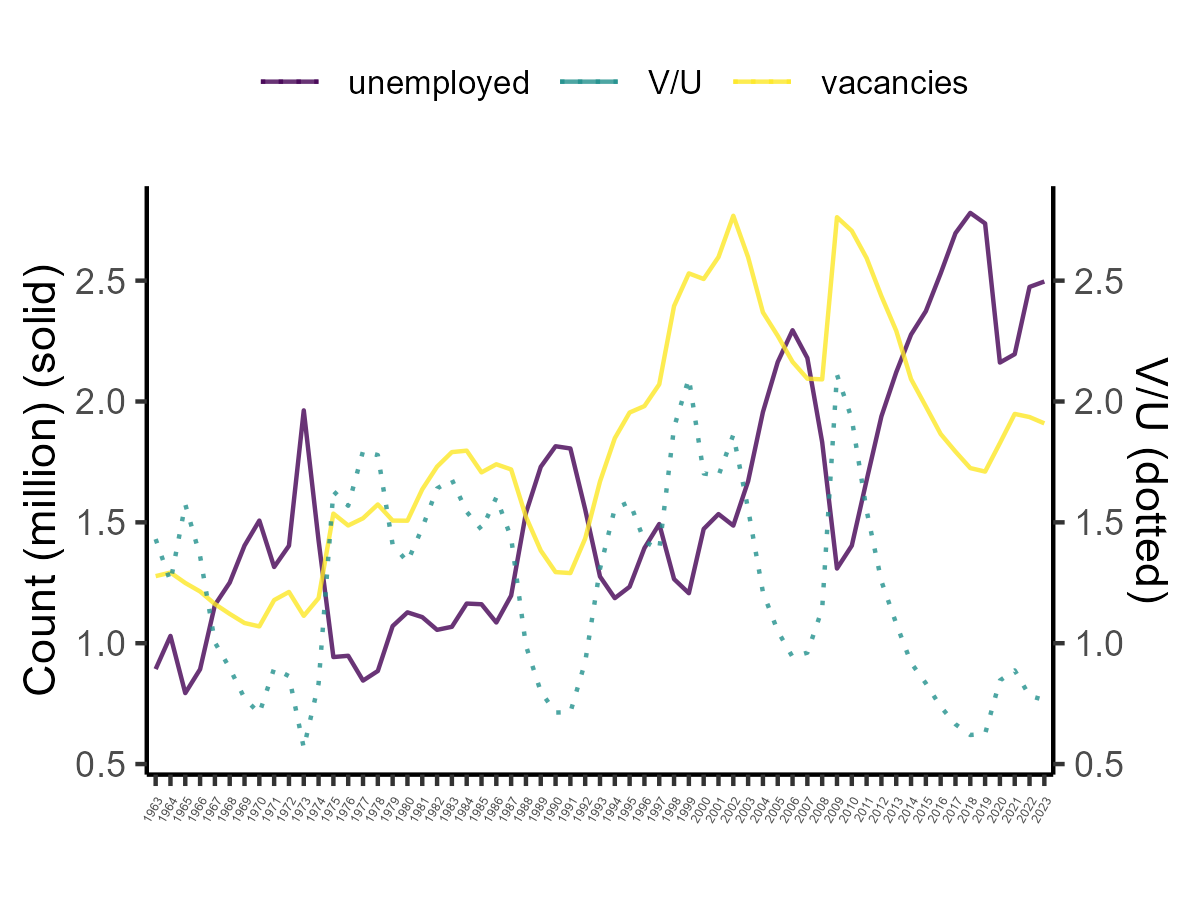
\includegraphics[width = 0.375\textwidth]
  {figuretable/unemployed_vacancy_year.png}}
  \subfloat[Hire ($H_{t}$)]{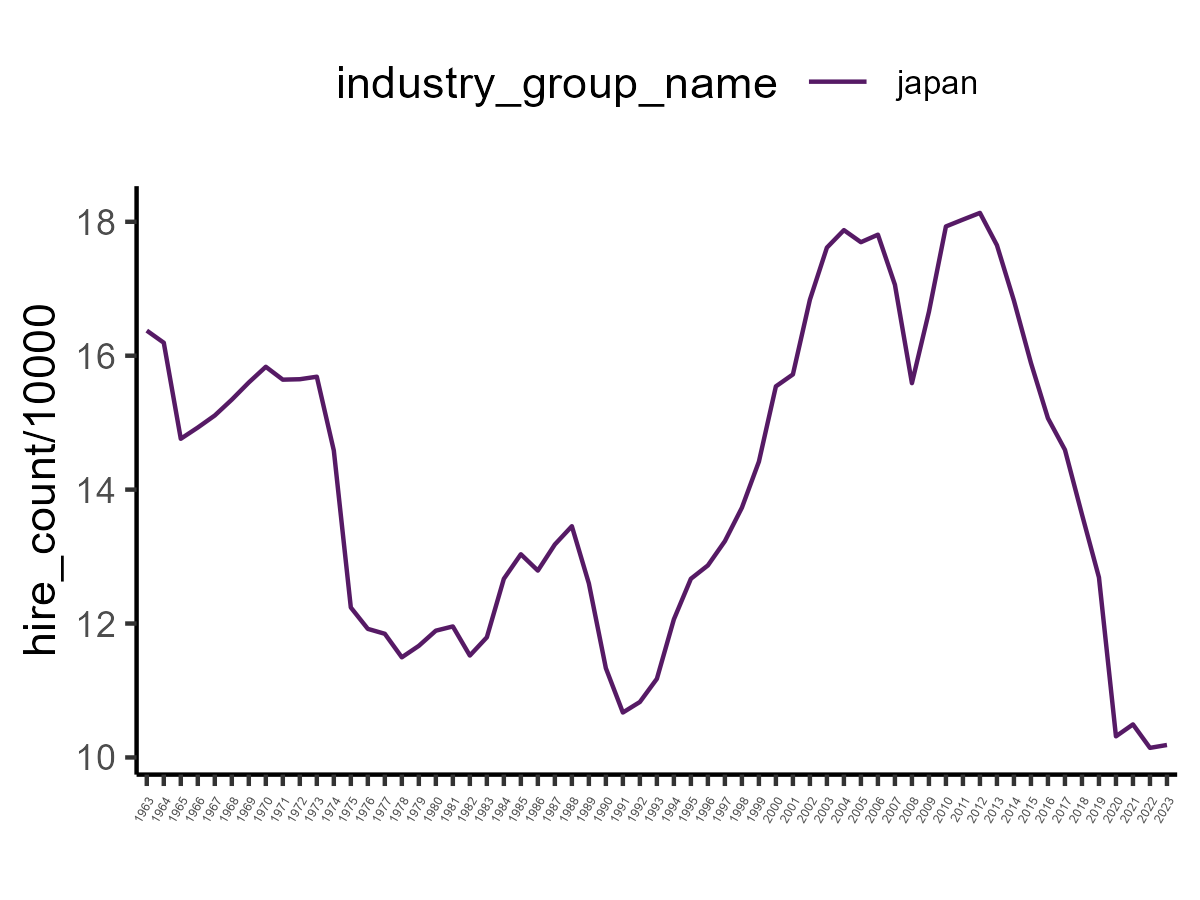
\includegraphics[width = 0.375\textwidth]
  {figuretable/hire_year.png}}\\
  \subfloat[Beveridge Curve ($U_{t}$ and $V_{t}$)]{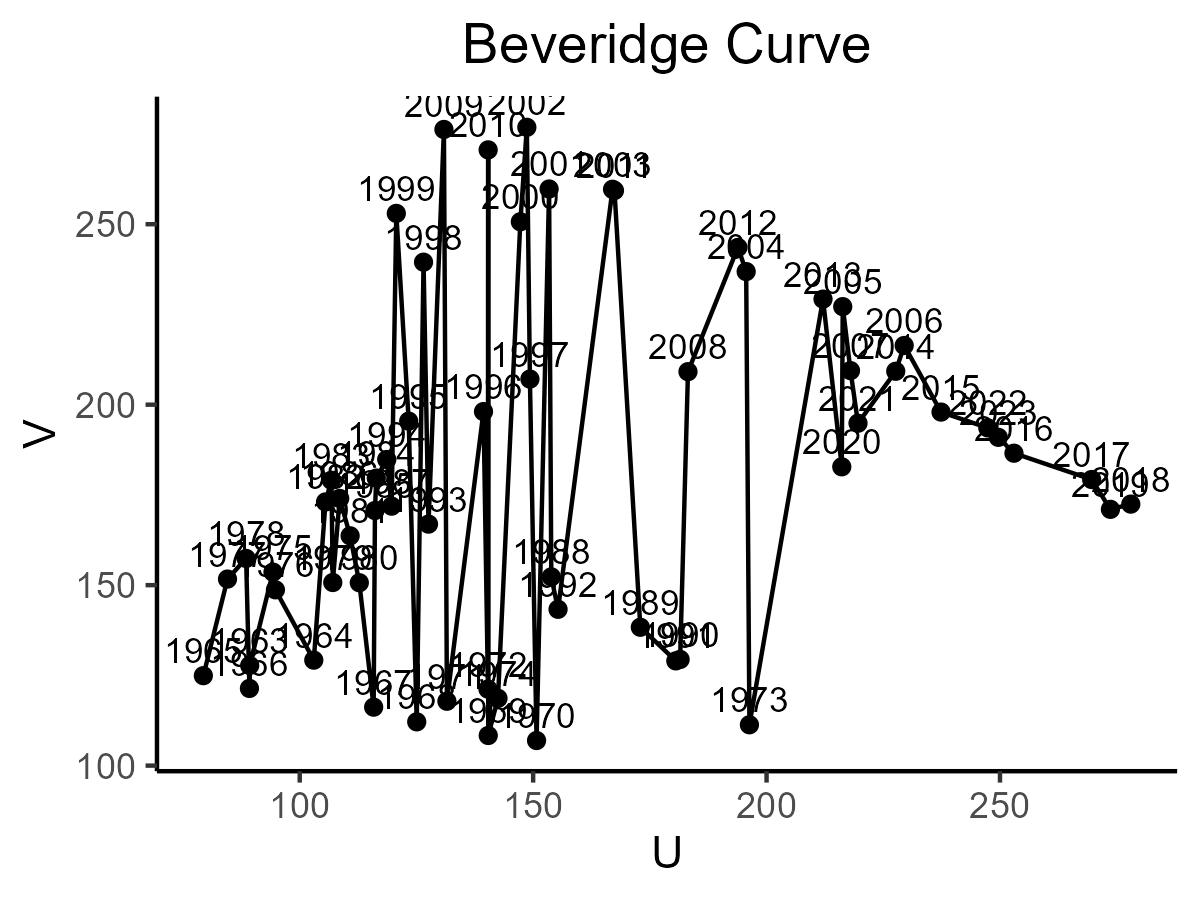
\includegraphics[width = 0.375\textwidth]
  {figuretable/unemployed_vacancies_berveridge_year.png}}
  \subfloat[Job finding rate ($\frac{M}{U}$) and Tightness  ($\frac{V}{U}$)]{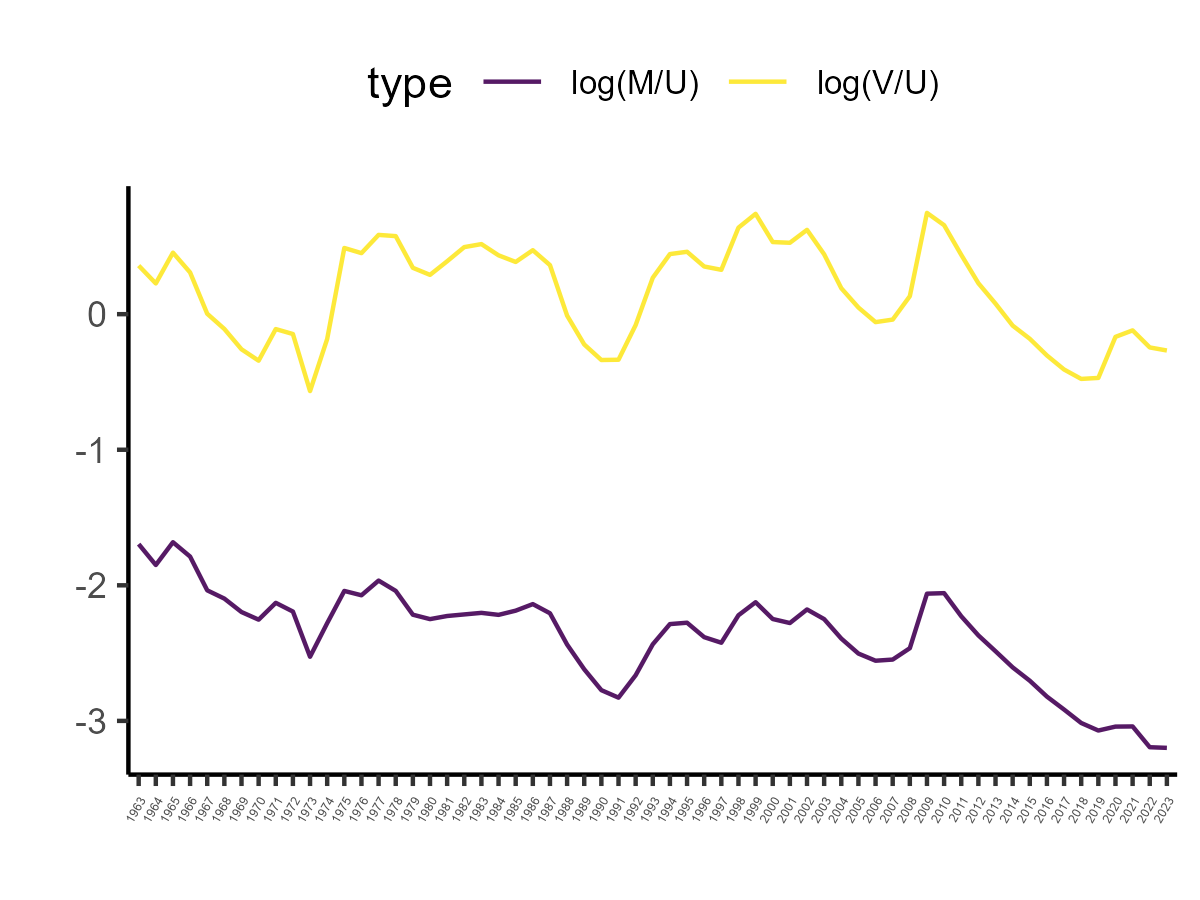
\includegraphics[width = 0.375\textwidth]
  {figuretable/job_finding_rate_tightness_year.png}}
  \\
  \subfloat[Matching Efficiency ($A_{t}$)]{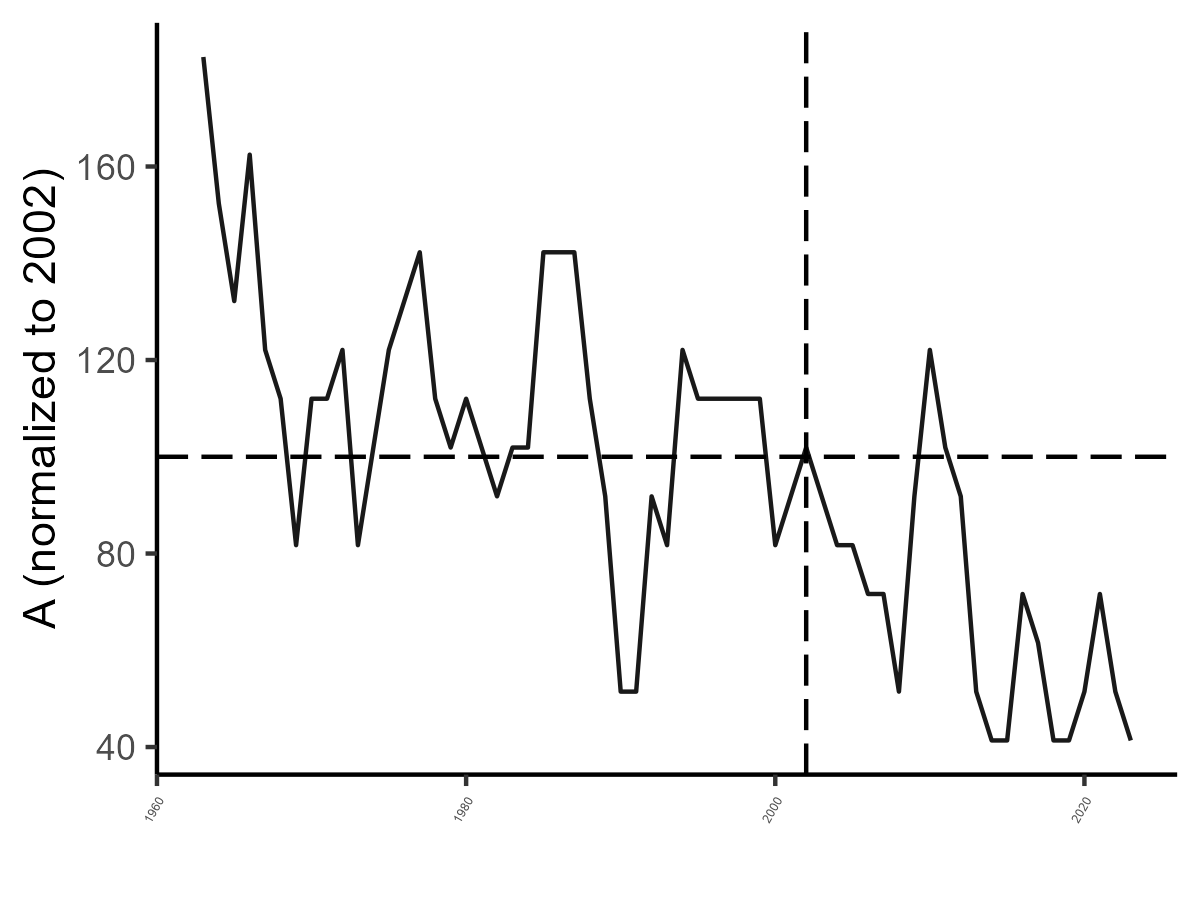
\includegraphics[width = 0.375\textwidth]
  {figuretable/matching_efficiency_year.png}}
  \subfloat[Matching Elasticity ($\frac{dM}{dU}$ and $\frac{dM}{dV}$)]{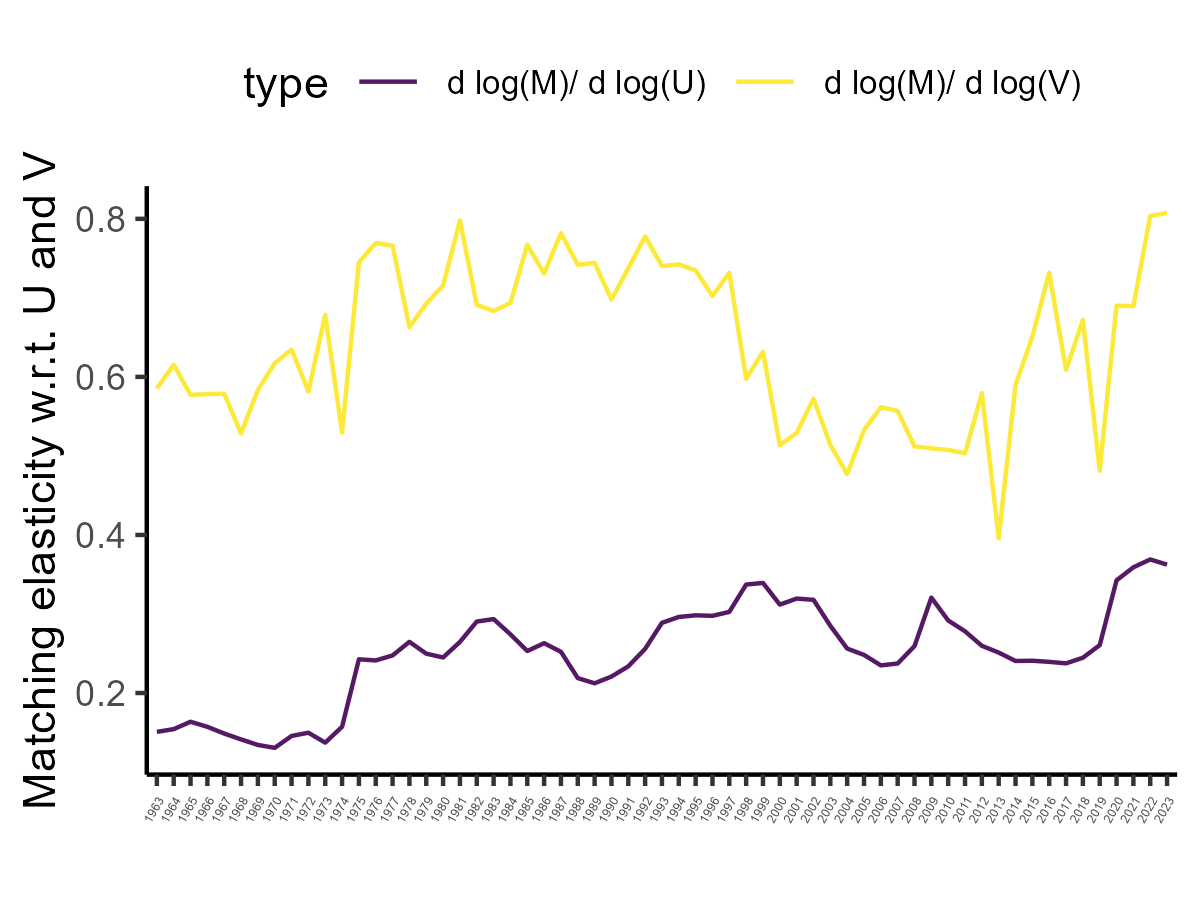
\includegraphics[width = 0.375\textwidth]
  {figuretable/elasticity_year.png}}\\
  \subfloat[Efficiency ($A$) and Tightness ($\frac{V}{U}$)]{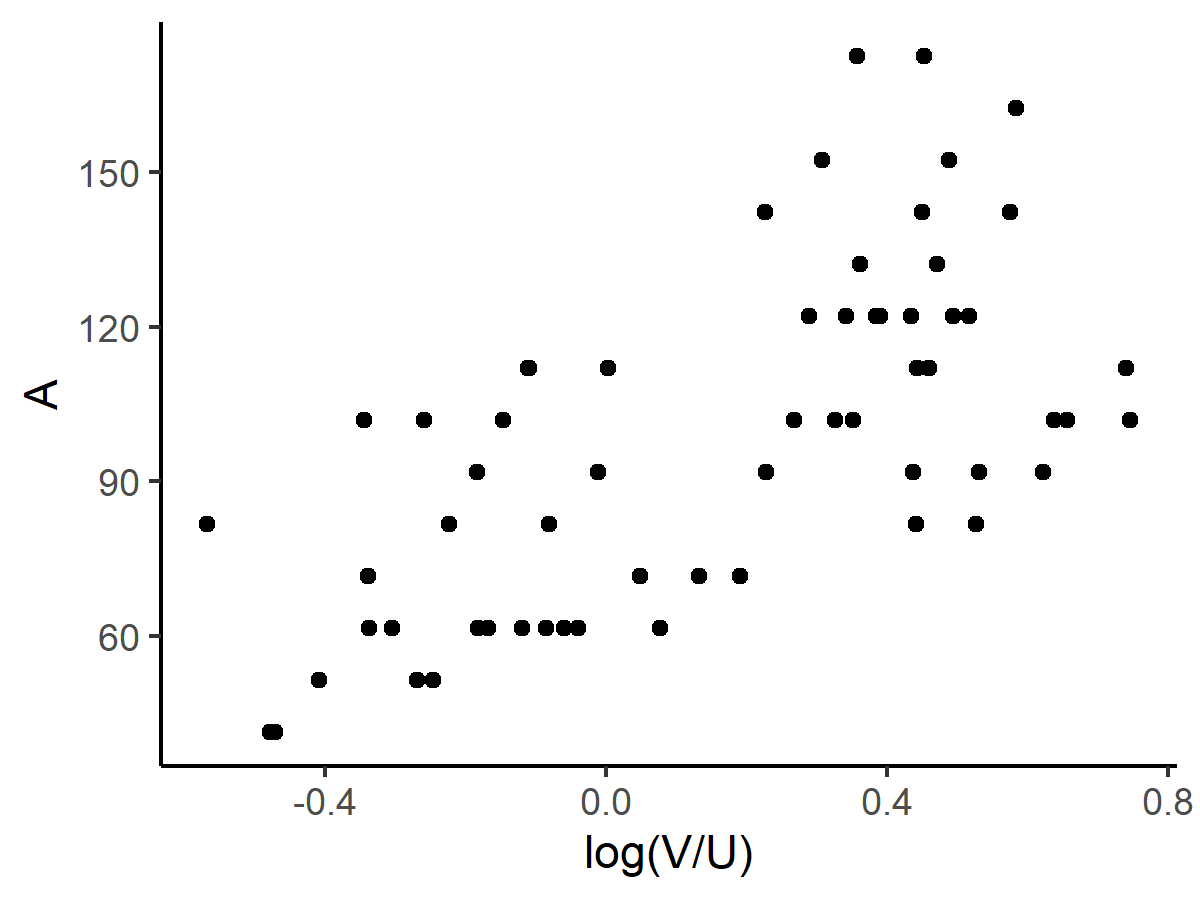
\includegraphics[width = 0.375\textwidth]
  {figuretable/efficiency_tightness_plot_year.png}}
  \subfloat[Efficiency ($A$) and ($\frac{M}{U}$, $\frac{M}{V}$)]{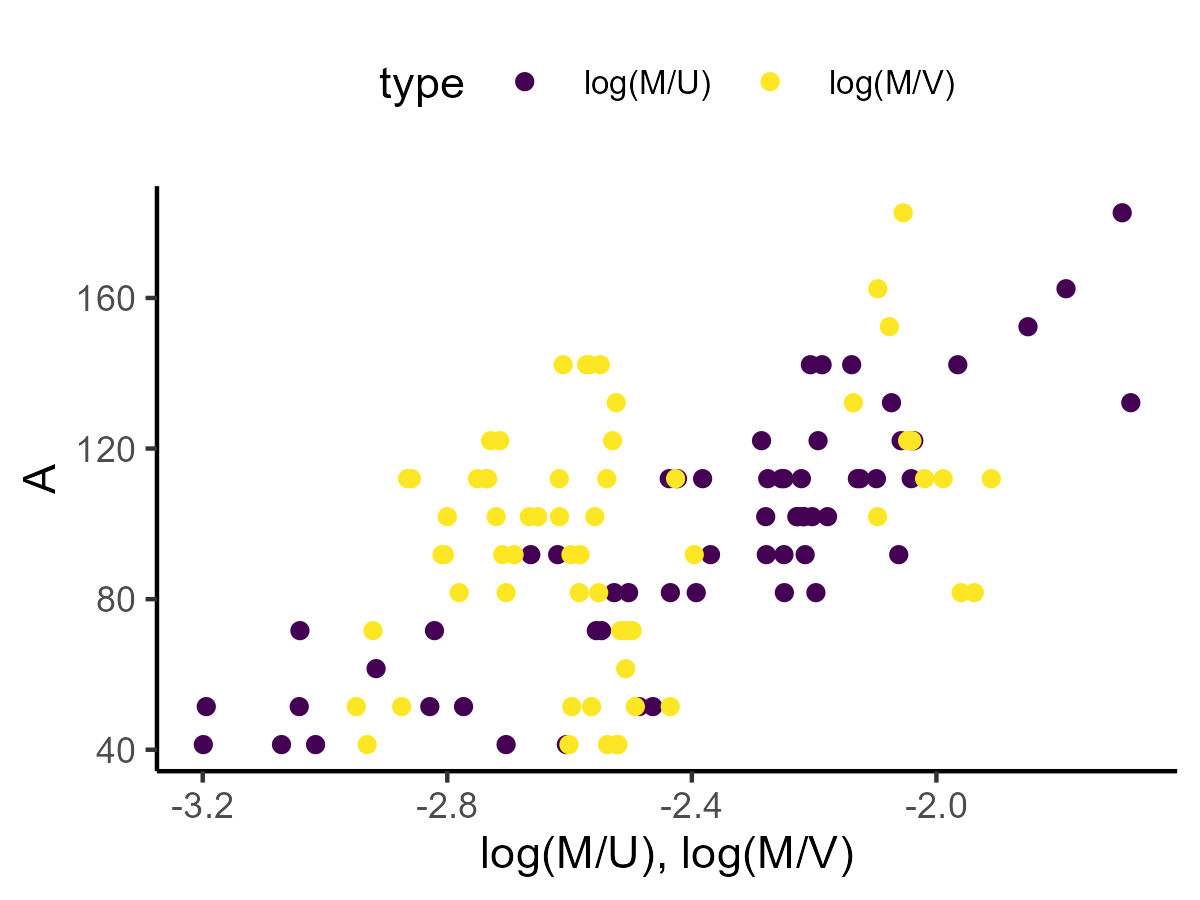
\includegraphics[width = 0.375\textwidth]
  {figuretable/job_finding_rate_efficiency_plot_year.png}}
  \caption{Year-level results}
  \label{fg:year_level_results} 
  \end{center}
  \footnotesize
  %Note: 
\end{figure} 


\subsection{Month-level trends in 1966-2023}

Figures \ref{fg:month_level_results} provide a month-level counterpart of Figure \ref{fg:year_level_results}. 
Note that I normalize matching efficiency at 2002 January to 100 for comparison across Figure \ref{fg:month_level_results} and Figure \ref{fg:year_level_results}.
General data patterns are consistent with year-level ones except for the existence of fluctuations.
Figures \ref{fg:month_level_results} (e) and (f) show estimation results of the matching function along with matching efficiency and elasticities.
Figures \ref{fg:month_level_results} (g) and (h) illustrate some correlation patterns between matching efficiency and market structure such as labor market tightness, job filling rate, and job finding rate.

\begin{figure}[!ht]
  \begin{center}
 \subfloat[Unemployed ($U_{t}$) and Vacancy ($V_{t}$)]{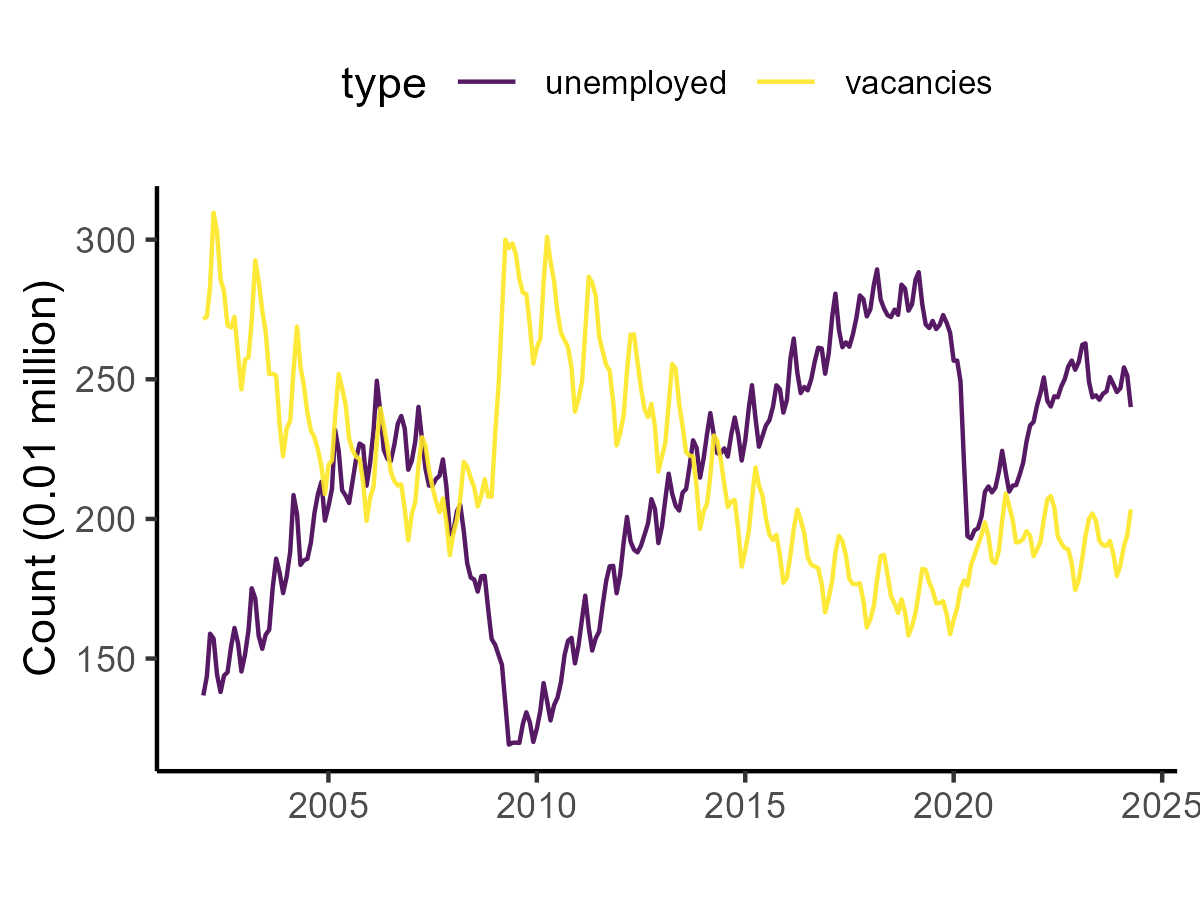
\includegraphics[width = 0.375\textwidth]
  {figuretable/unemployed_vacancy_month.png}}
  \subfloat[Hire ($H_{t}$)]{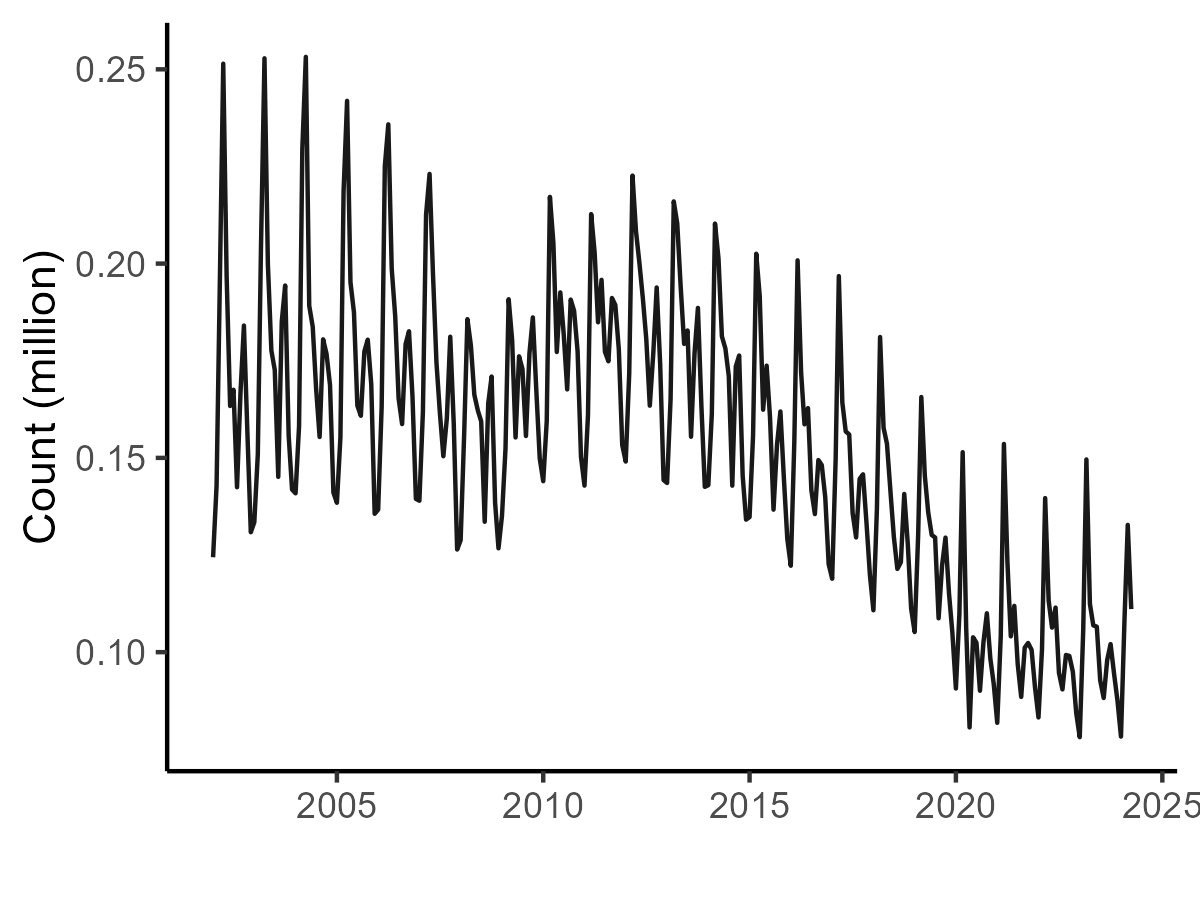
\includegraphics[width = 0.375\textwidth]
  {figuretable/hire_month.png}}\\
  \subfloat[Beveridge Curve ($U_{t}$ and $V_{t}$)]{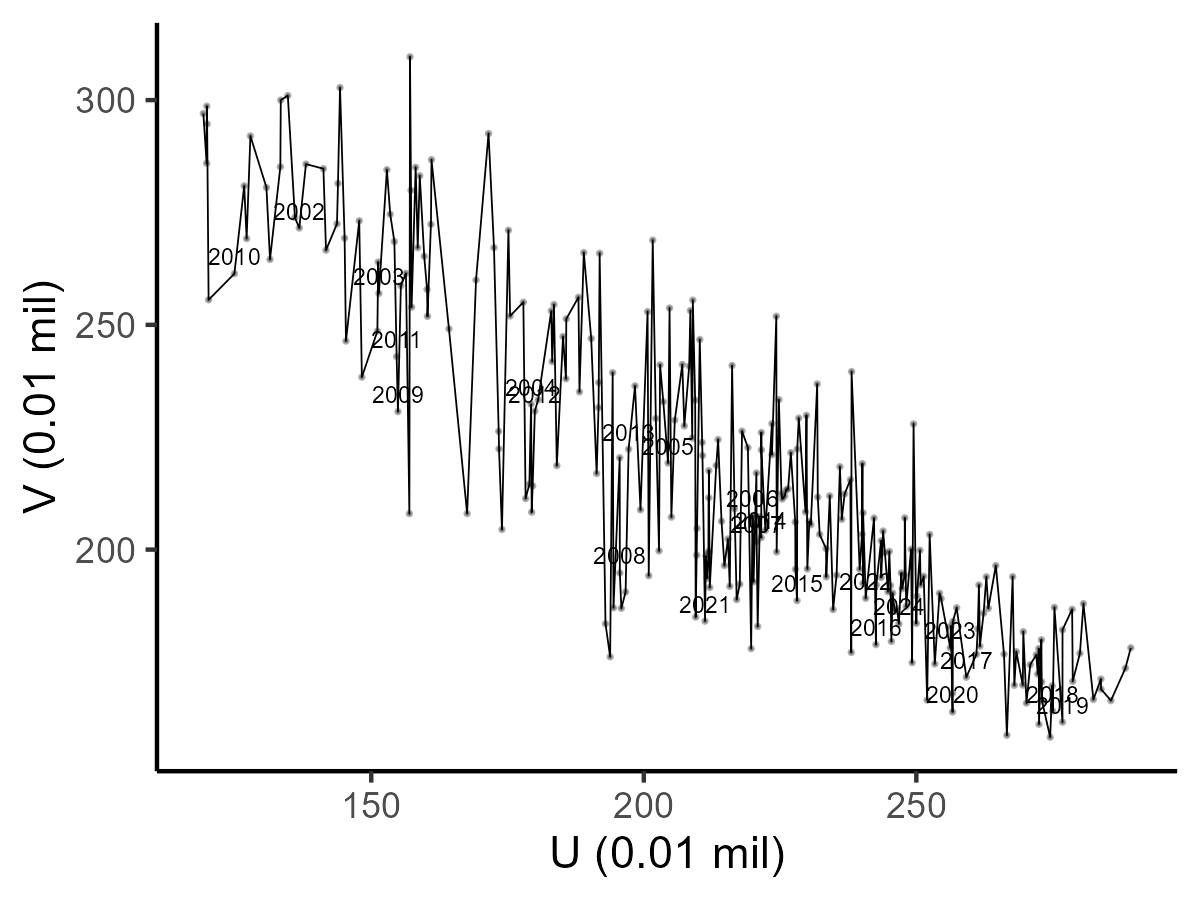
\includegraphics[width = 0.375\textwidth]
  {figuretable/unemployed_vacancies_berveridge_month.png}}
  \subfloat[Job finding rate ($\frac{M}{U}$) and Tightness ($\frac{V}{U}$)]{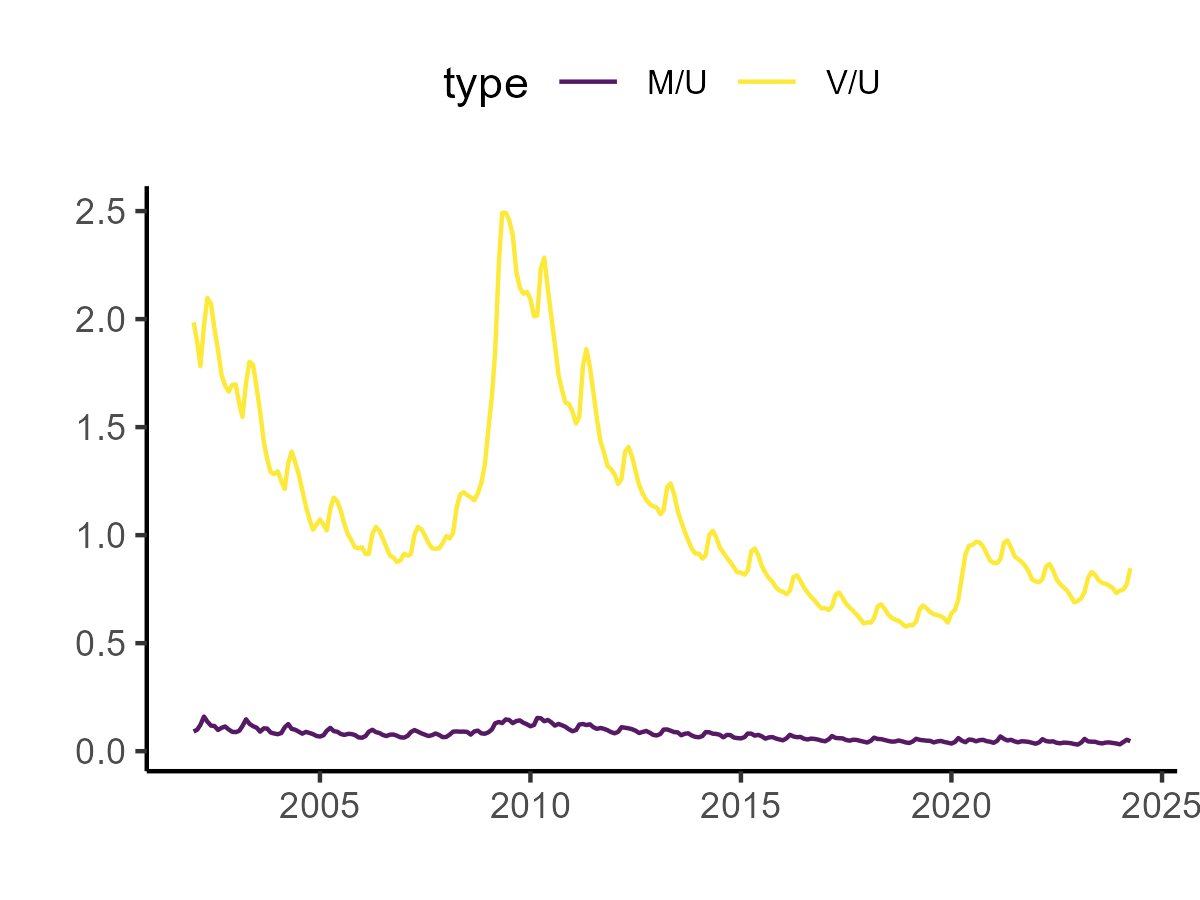
\includegraphics[width = 0.375\textwidth]
  {figuretable/job_finding_rate_tightness_month.png}}
  \\
  \subfloat[Matching Efficiency ($A_{t}$)]{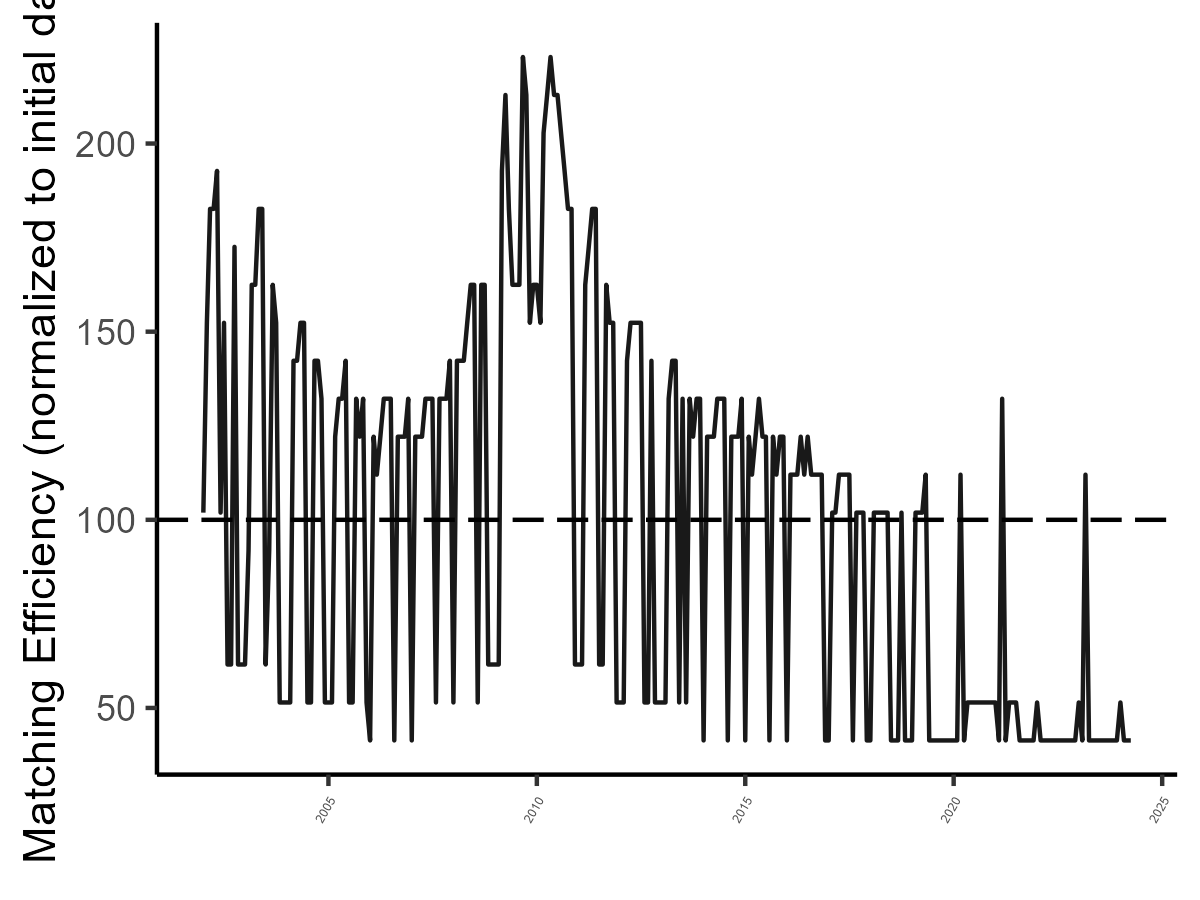
\includegraphics[width = 0.375\textwidth]
  {figuretable/matching_efficiency_month.png}}
  \subfloat[Matching Elasticity ($\frac{dM}{dU}$ and $\frac{dM}{dV}$)]{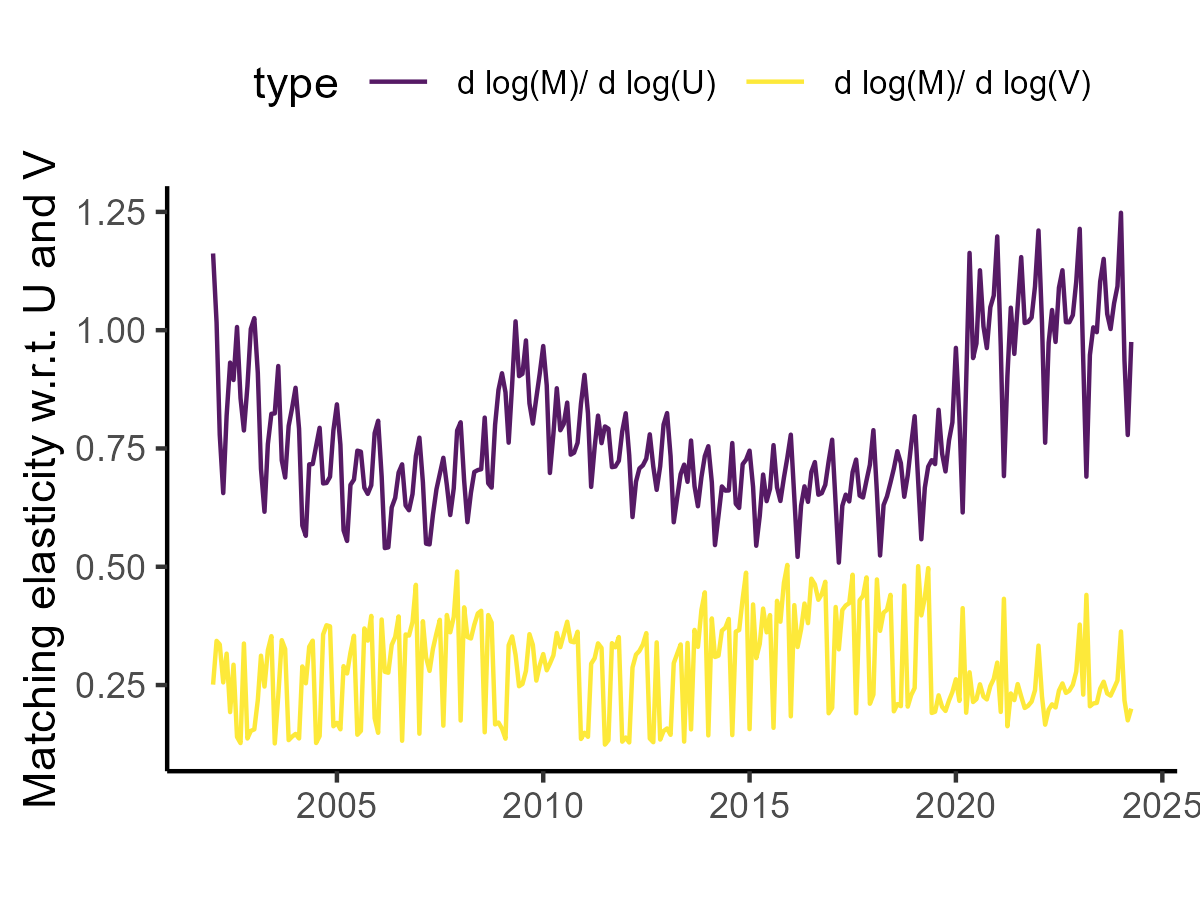
\includegraphics[width = 0.375\textwidth]
  {figuretable/elasticity_month.png}}\\
  \subfloat[Efficiency ($A$) and Tightness ($\frac{V}{U}$)]{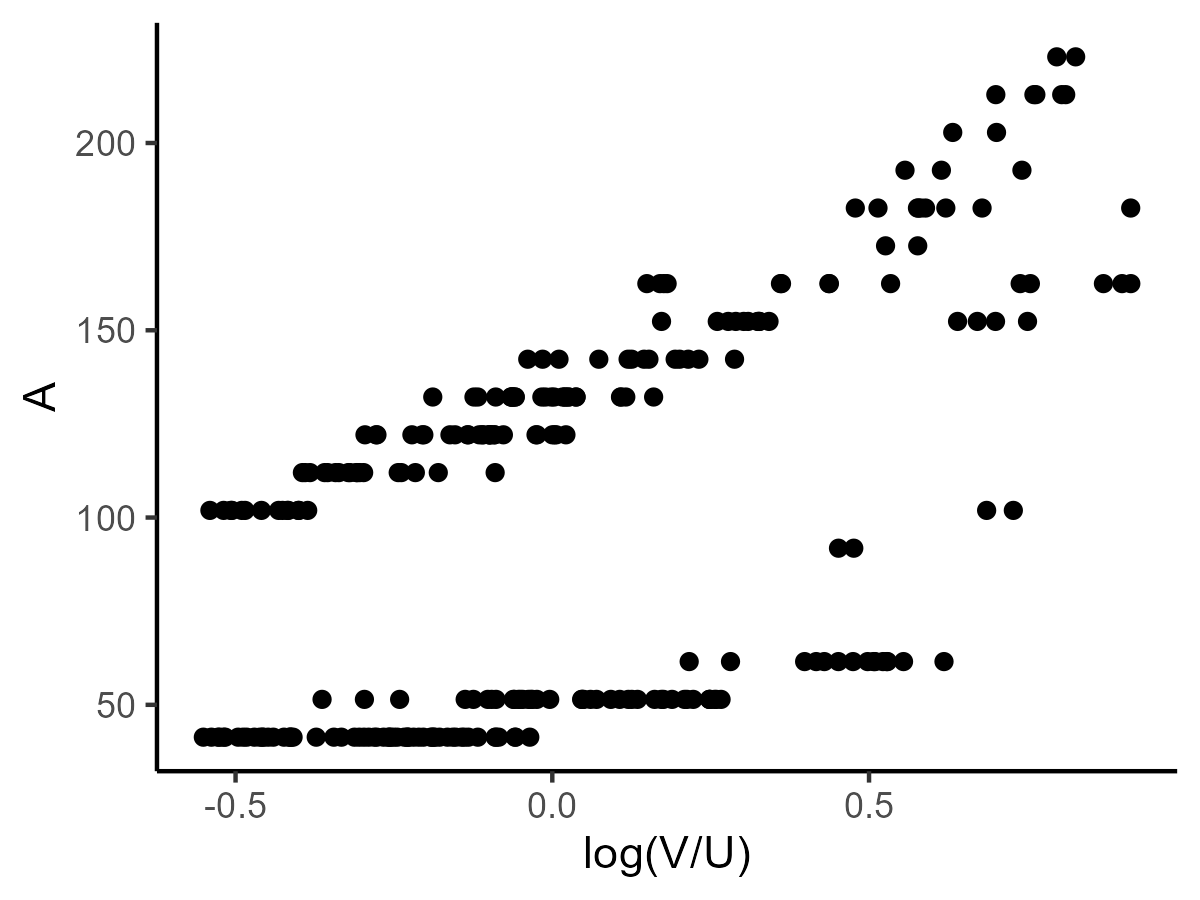
\includegraphics[width = 0.375\textwidth]
  {figuretable/efficiency_tightness_plot_month.png}}
  \subfloat[Efficiency ($A$) and ($\frac{M}{U}$, $\frac{M}{V}$)]{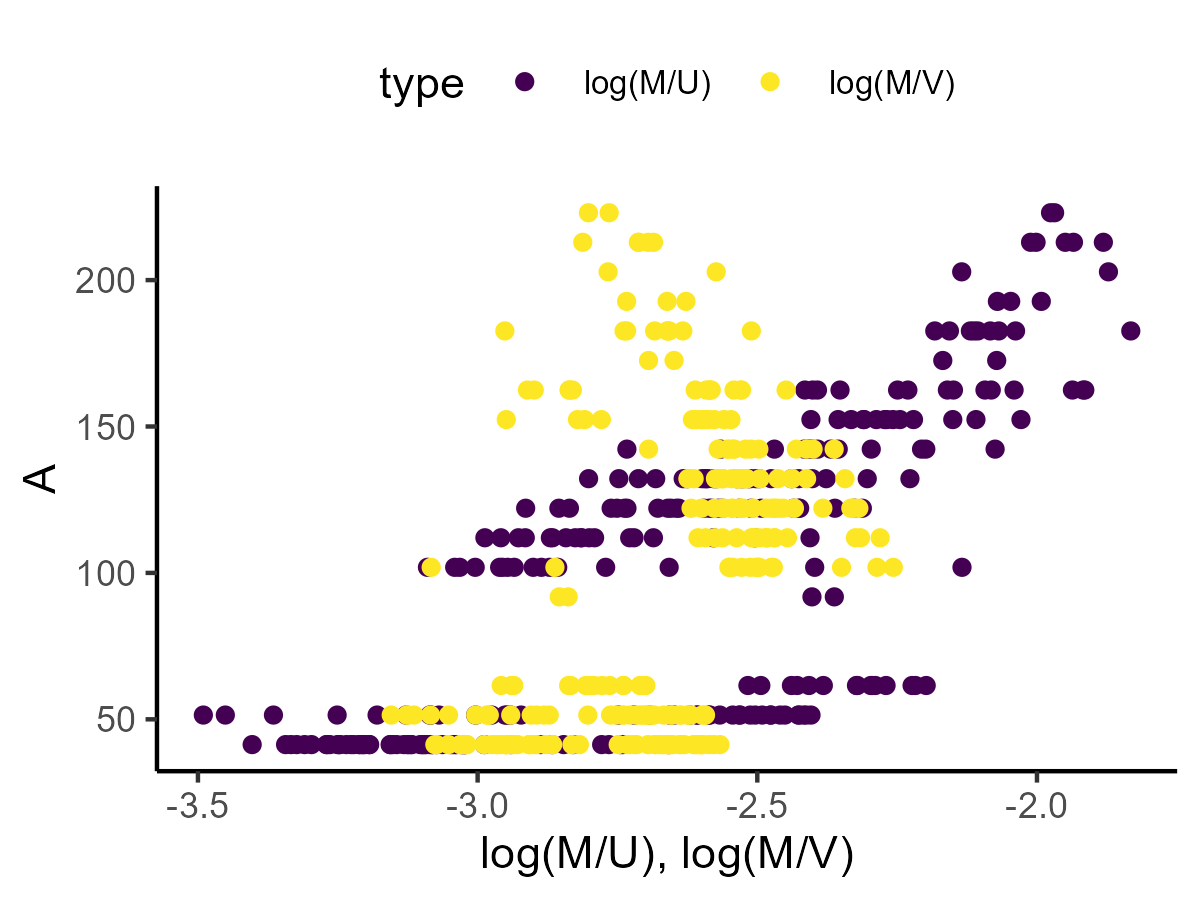
\includegraphics[width = 0.375\textwidth]
  {figuretable/job_finding_rate_efficiency_plot_month.png}}
  \caption{Month-level results}
  \label{fg:month_level_results} 
  \end{center}
  \footnotesize
  %Note: 
\end{figure} 


\section{Conclusion}

aa


\paragraph{Acknowledgments}
I thank Fuhito Kojima, Kosuke Uetake, Akira Matsushita, Kazuhiro Teramoto for his valuable advice. \textcolor{blue}{This research did not receive any specific grant from funding agencies in the public, commercial, or not-for-profit sectors.[KAKENHI number]}



\bibliographystyle{ecca}
\bibliography{matching_function}

\end{document}









